\documentclass[preview]{standalone}

\usepackage{amsmath}
\usepackage{amssymb}
\usepackage{stellar}
\usepackage{definitions}
\usepackage{tikz}
\usepackage{wrapfig}
\usepackage{bettelini}

\begin{document}

\id{multivariable-optimization-exercises}
\genpage

\section{Exercies}

\begin{snippetexercise}{multivariable-optimization-ex-1}{}
    Determine the local extrema of the \function
    \[
        f(x,y) = x^2y - xy^2 + xy
    \]
\end{snippetexercise}

\begin{snippetsolution}{multivariable-optimization-ex-1-sol}{}
    The gradient is given by
    \[
        \gradient f = \begin{pmatrix}
            2xy - y^2 + y \\ x^2 - 2xy + x
        \end{pmatrix}
    \]
    the components are null when
    \begin{align*}
        \begin{cases}
            y(2x - y + 1) = 0 \\
            x(x-2y + 1) = 0
        \end{cases}
    \end{align*}
    meaning that the point \(P_1 = (0,0)\),
    \(P_2 = (-1,0)\), \(P_3 = (0,1)\) and \(P_4 = (-1/3, 1/3)\) are critical.
    The Hessian matrix is given by
    \[
        Hf = \begin{pmatrix}
            2y & 2x - 2y + 1 \\ 2x - 2y + 1 & -2x
        \end{pmatrix}
    \]
    At the four points we have
    \[
        Hf(P_1) = \begin{pmatrix}
            0 & 1 \\ 1 & 0
        \end{pmatrix}, \quad
        Hf(P_2) = \begin{pmatrix}
            0 & -1 \\ -1 & 2
        \end{pmatrix}, \quad
        Hf(P_3) = \begin{pmatrix}
            2 & -1 \\ -1 & 0
        \end{pmatrix}, \quad
        Hf(P_4) = \begin{pmatrix}
            \frac23 & -\frac13 \\ -\frac13 & \frac23
        \end{pmatrix}
    \]
    which yields the following characterizations:
    \begin{enumerate}
        \item[\(P_1\):] \(\det Hf(P_1) = -1\). One positive and one negative eigenvalue, meaning this is a saddle point;
        \item[\(P_2\):] \(\det Hf(P_2) = -1\). One positive and one negative eigenvalue, meaning this is a saddle point;
        \item[\(P_3\):] \(\det Hf(P_3) = -1\). One positive and one negative eigenvalue, meaning this is a saddle point;
        \item[\(P_4\):] \(\det Hf(P_4) = 3/9\). We have two positive eigenvalues,
        and \(\trace(Hf(P_4)) = 4/3>0\) meaning that it is a minimum.
    \end{enumerate}
\end{snippetsolution}

\begin{snippetexercise}{multivariable-optimization-ex-2}{}
    Determine the local extrema of the \function
    \[
        f(x,y) = \frac{1}{2}x^2y^2 - 2y^2 + \frac{1}{3}x^3
    \]
\end{snippetexercise}

\begin{snippetexercise}{multivariable-optimization-ex-3}{}
    Determine the local extrema of the \function
    \[
        f(x,y) = {(x-1)}^2 (x^2 - y^2)
    \]
\end{snippetexercise}

\begin{snippetexercise}{multivariable-optimization-ex-4}{}
    Determine the local extrema of the \function
    \[
        f(x,y) = \frac{x^3y}{3} + \frac{1}{2}x^2y + \frac{1}{2}y^2
    \]
\end{snippetexercise}

\begin{snippetexercise}{multivariable-optimization-ex-5}{}
    Determine the local extrema of the \function
    \[
        f(x,y) = x^2y(x-y+1)
    \]
\end{snippetexercise}

\begin{snippetexercise}{multivariable-optimization-ex-6}{}
    Determine the local extrema of the \function
    \[
        f(x,y) = xy{(1-x^2-y^2)}^2
    \]
\end{snippetexercise}

\begin{snippetsolution}{multivariable-optimization-ex-6-sol}{}
    We first note that \(f(-x,y) = f(x,-y) = -f(x,y)\).
    The derivatives are given by
    \[
        f_x = y(1-x^2-y^2)(1-5x^2-y^2), \quad
        f_y = x(1-x^2-y^2)(1-x^2 - 5y^2)
    \]
    The partial derivatives are null when
    \[
        \begin{cases}
            y(1-x^2-y^2)(1-5x^2-y^2) = 0\\
            x(1-x^2-y^2)(1-x^2 - 5y^2) = 0
        \end{cases}
    \]
    This yields the following equations
    \[
        y = 0 \\
        x(1-x^2)(1-x^2) = 0
    \]
    which is satisfied at \((0,0), (\pm 1,0)\).
    Then, \(1-x^2-y^2 = 0\) yields the unitary circumference.
    Finally,
    \[
        \begin{cases}
            1 - 5x^2-y^2 = 0 \\
            x(4x^2)(-4+24x^2) = 0
        \end{cases}
    \]
    yields the points \((0, \pm 1)\), \(\pm 1 / \sqrt{6}, \pm 1 / \sqrt{6}\) and
    \((\pm 1 / \sqrt{6}, \mp 1 / \sqrt{6})\).
    The mixed derivatives are
    \begin{align*}
        f_{xx} &= y\left((1-x^2-y^2)(-12x) + 8x^3\right) \\
        f_{yy} &= -2xy(6-6x^2 - 10y^2) \\
        f_{xy} &= (1-x^2-y^2)(1-5x^2 - y^2)-4y^2(1-3x^2-y^2)
    \end{align*}
    At the origin we have
    \[
        \hessian_f(0,0) = \begin{pmatrix}
            0 & 1 \\ 1 & 0
        \end{pmatrix}
    \]
    which has \(\det \hessian_f(0,0) = -1 < 0\) and thus the origin is a saddle point.
    At the point \((1 / \sqrt{6}, 1 / \sqrt{6})\) we have
    \[
        \hessian_f\left(\frac{1}{\sqrt{6}}, \frac{1}{\sqrt{6}}\right) = \begin{pmatrix}
            -\frac{10}{9} & -\frac{2}{9} \\
            -\frac{2}{9} & -\frac{10}{9}
        \end{pmatrix}
    \]
    which has \(\det \hessian_f(1 / \sqrt{6}, 1 / \sqrt{6}) = 96/81 > 0\)
    and \(\trace \hessian_f(1 / \sqrt{6}, 1 / \sqrt{6}) = -20/9 < 0\).
    Thus, we have negative eigenvalues and this point is a maximum point.
    The same goes for \((-1 / \sqrt{6}, -1 / \sqrt{6})\)
    and the points \((1 / \sqrt{6}, -1 / \sqrt{6})\)
    and \((-1 / \sqrt{6}, 1 / \sqrt{6})\) are minimum points.
    \setlength{\intextsep}{0pt}%
    \begin{wrapfigure}{r}{3cm}
        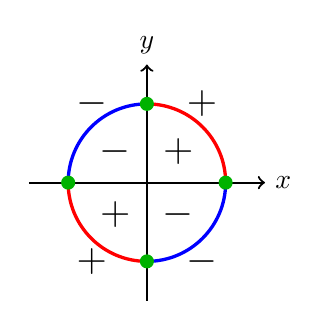
\begin{tikzpicture}[scale=1]
            % Axes
            \draw[->, thick] (-1.5,0) -- (1.5,0) node[right] {$x$};
            \draw[->, thick] (0,-1.5) -- (0,1.5) node[above] {$y$};

            % Circle arcs (alternating red/blue)
            \draw[very thick, red] (0:1) arc[start angle=0, end angle=90, radius=1];    % Q1 (+)
            \draw[very thick, blue] (90:1) arc[start angle=90, end angle=180, radius=1]; % Q2 (-)
            \draw[very thick, red] (180:1) arc[start angle=180, end angle=270, radius=1]; % Q3 (+)
            \draw[very thick, blue] (270:1) arc[start angle=270, end angle=360, radius=1]; % Q4 (-)

            % Signs outside the circle
            \node at (0.7,1.0) {\Large $+$};
            \node at (-0.7,1.0) {\Large $-$};
            \node at (-0.7,-1.0) {\Large $+$};
            \node at (0.7,-1.0) {\Large $-$};

            % Signs inside the circle
            \node at (0.4,0.4) {\Large $+$};
            \node at (-0.4,0.4) {\Large $-$};
            \node at (-0.4,-0.4) {\Large $+$};
            \node at (0.4,-0.4) {\Large $-$};

            % Small circles at the "corner" points
            \foreach \x/\y in {1/0, 0/1, -1/0, 0/-1}{
            \draw[thick, green!70!black, fill] (\x,\y) circle (0.075);
            }
        \end{tikzpicture}
    \end{wrapfigure}
    We know that the same criterion does not work for a curve of critical points.
    We thus study \(f\) on neighbhoords of the unitary circumference.
    By the study of the graph we can see that
    the {\color{green!70!black}points} \((\pm, 0), (0, \pm 1)\)
    are saddle points. The {\color{red}points}
    \[
        \left(S^1 \intersection \{(x,y) \in \realnumbers^2 \suchthat x>0\land y>0\}\right)
        \union
        \left(S^1 \intersection \{(x,y) \in \realnumbers^2 \suchthat x<0\land y<0\}\right)
    \]
    are maximum points and the {\color{blue}points}
    \[
        \left(S^1 \intersection \{(x,y) \in \realnumbers^2 \suchthat x>0\land y<0\}\right)
        \union
        \left(S^1 \intersection \{(x,y) \in \realnumbers^2 \suchthat x<0\land y>0\}\right)
    \]
    are minimum points.
    \wrapfill
\end{snippetsolution}

\begin{snippetexercise}{multivariable-optimization-ex-7}{}
    Determine the local extrema of the \function
    \[
        f(x,y) = \frac{x^2 + 2y}{x^2 + y^2 + 1}
    \]
\end{snippetexercise}

\begin{snippetsolution}{multivariable-optimization-ex-7-sol}{}
    We first note that
    \[
        f(x,y) = \frac{x^2 + 2y + 1}{x^2 + y^2 + 1} + \frac{x^2 + 2y - 1}{x^2 + y^2 + 1}
        = 1 - \frac{{(y-1)}^2}{x^2 + y^2 + 1} \leq 1
    \]
    The partial derivatives are given by
    \[
        f_x = \frac{2x{(y-1)}^2}{{(x^2 + y^2 + 1)}^2}, \quad
        f_y = \frac{2(x^2 -y^2 + 1 -yx^2)}{{(x^2 + y^2 + 1)}^2}
    \]
    The partial derivatives are null at the points \((0, \pm 1)\)
    and at the line \((x, 1)\).
    The second partial derivates are
    \begin{align*}
        f_{xx} &= \frac{2{(y-1)}^2 (x^2 + y^2 + 1 - 4x^2)}{{(x^2 + y^2 + 1)}^3} \\
        f_{yy} &= \frac{2 \left[(-2xy - x^2)(x^2 + y^2 + 1) - 4y(x^2 - y^2 + 1 -yx^2)\right]}{{(x^2 + y^2 + 1)}^3} \\
        f_{xy} &= \frac{4x(y-1)\left[x^2 + y^2 + 1 - 2y(y-1)\right]}{{(x^2 + y^2 + 1)}^3}
    \end{align*}
    At the point \((0, -1)\) we have
    \[
        \hessian_f(0,-1) = \begin{pmatrix}
            2 & 0 \\ 0 & 1
        \end{pmatrix}
    \]
    which has \(\det H_f(0,-1) = 2 >\) and \(\trace H_f(0,-1) = 3>\), which means
    that this is a point of minimum.
    We will now study the point \((x,1)\).
    We know that the same criterion does not work for a curve of critical points.
    We have \(f(x,1) = 1\).
    Studying the sign in a neighbhoord of this point makes sense when \(f=0\). We thus
    translate the function \(g = f-1\). We have
    \[
        g(x,y) = \frac{x^2 + 2y - x^2 - y^2 - 1}{x^2 + y^2 + 1} = -\frac{{(y-1)}^2}{x^2 + y^2 + 1} \leq 0
    \]
    Thus, the points \((x,1)\) are points of weak absolute maximum.
\end{snippetsolution}

\begin{snippetexercise}{multivariable-optimization-ex-8}{}
    Verify that the origin is a critical point for the \function[functions]
    \[
        f(x,y,z) = \sin^2(x-z) + y^2 - xyz
    \]
    and
    \[
        g(x,y,z) = \sin^2(x-z) + y^2 + y^2z
    \]
    and determine their nature.
\end{snippetexercise}

\begin{snippetsolution}{multivariable-optimization-ex-8-sol}{}
    We have the derivatives
    \[
        g_x = 2\sin(x-z)\cos(x-z),
        \quad
        g_y = 2y(1+z),
        \quad
        g_z = -2\sin(x-z)\cos(x-z) + y^2
    \]
    and we have
    \[
        g_x(0,0,0) = g_y(0,0,0) = g_z(0,0,0)
    \]
    and thus the origin is a critical point.
    We now consider the second order partial derivatives
    \begin{align*}
        g_{xx} &= 2\cos(2u) \quad g_{xz} &= -2\cos(2u)\quad  g_{zz} &= 2\cos(2u)
        g_{yy} &= 2(1+z) \quad g_{yz} &= 2y g_{xy}\quad  &= 0
    \end{align*}
    with \(u = x-z\). We have
    \[
        \hessian(0,0,0) = \begin{pmatrix}
            2&0&-2\\0&2&0\\-2&0&2
        \end{pmatrix}
    \]
    Since \(\det H(0,0,0) = 0\) the test is inconclusive.
    Consider the parametrization \(g(t,0,t) = \sin^2(x-z) = 0\).
    We can note that \(g = \sin^2(x-z) + y^2 + y^2z = \sin^2(x-z) + y^2(1+z) \geq 0\)
    in a neighbhoord of \(0\). Thus the origin is a local minimum. \\
    For the other function we have
    \[
        f_x = 2\sin(x-z)\cos(x-z) - 4z,
        \quad
        f_y = 2y-xz,
        \quad
        f_z = -2\sin(x-z)\cos(x-z)-xy
    \]
    and we have
    \[
        f_x(0,0,0) = f_y(0,0,0) = f_z(0,0,0)
    \]
    and thus the origin is a critical point.
    We can parametrize \(g(x,y) = f(x,y,x) = y^2 - x^2y\).
    In a \neighborhood of the origin,
    \(g(0,y) = y^2 >0\) for \(y\neq 0\),
    and \(g(x, x^2/2) = -x^4 /4 < 0\) for \(x \neq 0\).
    Thus, in some directions the \function is increasing and in some it is decreasing,
    meaning that the point is a saddle point.
\end{snippetsolution}

\end{document}